\documentclass[11pt, a4paper, oneside]{article}

\usepackage[francais]{babel}
\usepackage[T1]{fontenc}
\usepackage[utf8]{inputenc}

\usepackage[left=2cm, right=2cm, top=2cm, bottom=2cm]{geometry}
\usepackage{fancyhdr}
\usepackage{lastpage}
\usepackage{hyperref}

\usepackage{graphicx}
\usepackage{tikz}
\usepackage{pgfgantt}

\usepackage{perpage} %the perpage package
\MakePerPage{footnote} %the perpage package command

\usepackage{color}
\usepackage{colortbl}

\usepackage{makeidx}

\usepackage{listings}
\usepackage{CJKutf8}

\usepackage{tabularx}

\makeindex
\makeatletter
\renewenvironment{theindex}
{
    \thispagestyle{fancy}
    \setlength{\parindent}{0pt}
    \let
    \item
    \@idxitem
}{\onecolumn}
\makeatother

\setlength{\parindent}{0cm}

\lstset{
    basicstyle=\ttfamily,
    stringstyle=\ttfamily\color{green!50!black},
    keywordstyle=\bfseries\color{blue},
    commentstyle=\itshape\color{red!50!black},
    showstringspaces=true,
    tabsize=4,
    frame=single,
    numbers=left,
    numberstyle=\tiny,
    firstnumber=1,
    stepnumber=1,
    numbersep=5pt,
    breaklines=true
}

\graphicspath{{img/}}

\pagestyle{fancy}
\setlength{\headheight}{14pt}
\renewcommand{\headrulewidth}{0.5pt}
\lhead{Yannick Brodard}
\chead{Travail de semestre}
\rhead{\today}
\renewcommand{\footrulewidth}{0.5pt}
\lfoot{CFPT - École d'informatique}
\cfoot{Étude de Unreal Engine 4}
\rfoot{Page \thepage ~sur \pageref{LastPage}}

% Niveau table des matières
\setcounter{tocdepth}{3}
% ---------------------------------------------------------------------
\begin{document}
\begin{center}
{\Huge{Étude de Unreal Engine 4}} \\[0.5cm]
{\LARGE{Travail de semestre}}\\[0.5cm]
{\Large{Yannick \textsc{Brodard}}}\\[0.3cm]
\today\\
\includegraphics[scale=0.4]{UE4_logo}
\end{center}
Enseignants :
\begin{itemize}
\item Christophe \textsc{Maréchal}
\item Stéphane \textsc{Garchery}\\[3cm]
\end{itemize}
\textbf{CFPT - École d'informatique}\\
Technicien ES 2\textsuperscript{ème} année
\thispagestyle{empty}
\newpage
\vspace*{\fill}
\begin{flushright}
\textit{Every good idea borders on the stupid.}\\[0.3cm]
- Michel \textsc{Gondry}
\end{flushright}
\vspace*{\fill}
\thispagestyle{empty}
\newpage
\part{Avant-propos}
\section{Résumé}
% A COMPLETER A LA FIN
\section{Remerciements}
% A COMPLETER A LA FIN
\newpage
\tableofcontents
\newpage
\part{Introduction}
\section{Définition du projet}
Ce projet a été mis en place pour s'initier au développement de jeux-vidéos avec un moteur de jeu, étant donné que mon travail de diplôme sera de développer un jeu complet.

Pour ce faire, une étude et un travail pratique avec l'environnement Unreal Engine 4 a été proposé.

Dans cette étude, plusieurs aspects de ce moteur seront analysés et documentés, notamment :
\begin{itemize}
\item La gestion des modèles 3D
\item La création de jeu
\item L'interaction utilisateur-machine\\
\end{itemize}
Proposé par Monsieur Maréchal, l'intégration d'un périphérique 3D (le \textit{Novint Falcon 3D Touch Controller}) a été prévu pour étudier son fonctionnement et son implémentation sur ce genre d'environnement.
\subsection{Unreal Engine 4}
\label{sec:ue4definition}
Unreal Engine est un moteur de jeu développé par Epic Games\footnote{\url{http://epicgames.com/}} qui a été présenté pour la première fois en 1998 avec un jeu FPS\footnote{First Person Shooter : Jeu de tir à la première personne} nommé \textit{Unreal}. Bien que le moteur était développé principalement pour des jeux FPS, il est aujourd'hui utilisé pour beaucoup d'autres genres de jeux comme :
\begin{itemize}
\item Infiltration
\item Action
\item MMO (Jeux massivement multijoueurs en-ligne)
\item Jeux à la troisième personne
\item Et bien d'autres...
\end{itemize}
La version actuelle de UE4\footnote{Unreal Engine 4} est conçu pour fonctionner avec Microsoft DirectX 10 à 12, OpenGL et JavaScript/WebGL.
\newpage
\section{Définition des objectifs}
Le but est d'étudier l'environnement de Unreal Engine 4 dans ses détails, c'est-à-dire la programmation avec UE4, la modélisation, l'édition de différents scénarios et prise en main de la physique du moteur. Un travail avec la souris \textit{Novint Falcon 3D Touch Controller} est aussi demandé, cette souris 3D permet à l'utilisateur de reproduire des mouvement sur 3 axes qui peuvent être interprétés par l'ordinateur.

\begin{figure}[h]
	\begin{center}
	\includegraphics[scale=.4]{falcon}
	\caption{Souris Novint Falcon 3D Touch Controller}
	\end{center}
\end{figure}

Une étude comparative du moteur de jeu sera faite avec le moteur Unity 3D, cette étude est confiée à Monsieur Daniel Lopes.\\[0.3cm]
Le mini-jeu est basé sur le jeu \textit{Galaga}. Dans ce jeu 2D, l'utilisateur contrôle un vaisseau qui peut se déplacer sur les axes x et y. Des vagues de vaisseaux ennemis se positionnent devant le joueur pour tenter de l'éliminer. Ils se positionnent en groupe et tirent sur le joueur. Le joueur doit faire de son mieux pour esquiver les tirs et doit détruire tous ses ennemis.

\begin{figure}[h]
	\begin{center}
	\includegraphics[scale=0.8]{Galaga}
	\caption{Capture d'écran du jeu Galaga}
	\end{center}
\end{figure}

\newpage
\part{Analyse préliminaire}
\section{Analyse de l'existant}
Concernant le mini-jeu, il y a la plateforme et le moteur sur le quel celui-ci se repose. \mbox{Unreal Engine 4} permet de développer des jeux de manière beaucoup plus rapide et efficace sans ré-inventer la roue. Ceci permet d'éviter d'écrire des bibliothèques pour, par exemple, gérer l'affichage du jeu.

À propos du jeu en lui-même, il n'y a rien de codé ni préparé. Il y a la conception totale à faire.
\section{Environnement de travail}
\subsection{Logiciel}
\begin{itemize}
\item Unreal Engine 4\footnote{Pour en savoir plus sur Unreal Engine 4 voir la section \ref{sec:ue4definition} sur la page \pageref{sec:ue4definition}.}
\item Outils de Unreal Engine 4
\item Visual Studio Professional 2013\\
\end{itemize}
\subsection{Matériel}
\begin{itemize}
\item PC 1x
	\begin{itemize}
	\item 1024MB NVIDIA GeForce GTX 550 Ti
	\item Intel Core i7 2600K @ 3.40GHz
	\item ASUSTeK Computer INC. P8Z68-V LE
	\item 8.00 Go Dual-Channel DDR3 @ 824MHz
	\end{itemize}
\item Écran 2x
\item Clavier 1x
\item Souris 1x
\end{itemize}
\subsection{Conditions de travail}
\subsubsection{Durée}
Le projet se déroulera sur 48 heures de cours, séparée sur 12 jours et 4 périodes par jour. C'est-à-dire, une fois par semaine, le mercredi matin, 4 périodes seront dédiées à ce projet. Il est aussi possible de travailler sur le projet en dehors des ces tranches horaires.
\subsubsection{Délivrables}
\begin{itemize}
\item Un journal de bord
\item Une copie de la documentation
\item Un poster qui présente le projet
\item La documentation et la source du projet seront déposées sur la plateforme Moodle du CFPT-EI.
\end{itemize}
\subsubsection{Suivi}
Ce projet sera évalué et suivi par Monsieur Christophe Maréchal et Monsieur Stéphane Garchery.
\newpage
\part{Étude Unreal Engine 4}
\section{Unreal Editor}
\begin{center}
\begin{figure}[htp]
\includegraphics[scale=.39]{ue4editor}
\caption{Unreal Editor}
\end{figure}
\end{center}

\subsection{Bar de contrôle}
La bar de contrôle permet de gérer les points important du projet, comme la sauvegarde, le contenu, les \emph{blueprints}, la génération et la compilation (voir figure \ref{fig:bardecontrole}).

\begin{description}
	\item{\textbf{Save}} permet de sauvegarder le projet.
	\item{\textbf{Source Control}} vérifie l'intégrité du projet.
	\item{\textbf{Content}} affiche les contenus.
	\item{\textbf{Marketplace}} permet de naviguer dans la marché de UE4 pour télécharger du contenu.
	\item{\textbf{Settings}} permet de modifier les paramètres du projet.
	\item{\textbf{Matinee}} permet de gérer les animations.
	\item{\textbf{Build}} génère votre projet.
	\item{\textbf{Compile}} compile votre code C++ pour l'éditeur.
	\item{\textbf{Play}} permet de jouer directement sur l'éditeur.
	\item{\textbf{Launch}} permet de générer la version finale du produit.
\end{description}

\begin{center}
\begin{figure}[htp]
\includegraphics[scale=.8]{bardecontrole}
\caption{Bar de contrôle de l'éditeur}
\label{fig:bardecontrole}
\end{figure}
\end{center}

\subsection{Blueprints (Plans)}
Les \emph{Blueprints} sont des plans qui permettent d'ajouter des fonctionnalités à un objet ou une classe sans devoir passer par du code C++.\\[.4cm]
\textbf{Exemple - Configuration d'une caméra statique}
\begin{center}
\begin{figure}[htp]
\includegraphics[scale=.8]{blueprint}
\caption{\emph{Blueprint} du niveau pour fixer une caméra statique}
\label{fig:blueprint}
\end{figure}
\end{center}

Avec l'éditeur de \emph{Blueprint}, il est possible de placer directement des fonctions, des actions et des méthodes dans cette interface graphique afin de produire du code pour le jeu (Voir figure \ref{fig:blueprint}).

\emph{Event Begin Play} est la méthode de démarrage et action une fonction \emph{Set View Target with Blend} qui permet de mettre en place la caméra utilisée par le jeu. \emph{Get Player Controller} est un \emph{getter} qui permet de récupérer le contrôleur du joueur, il est ensuite lié à la cible \emph{target} de la fonction. La caméra de notre scène est lié comme cible pour la vue par défaut.

Il est ainsi possible grâce à l'utilisation de \emph{Blueprints} de programmer un jeu complet sans toucher au code.

\newpage

\subsection{Mesh (Maillage)}
Le système de maillage est le squelette de votre objet (ou personnage). Il permet de lui donner des logiques de collision et d'animation.

\begin{center}
\begin{figure}[htp]
\includegraphics[scale=.47]{mesh}
\caption{\emph{Matinee} est l'outil utilisé pour l'édition des \emph{meshes}}
\label{fig:mesh}
\end{figure}
\end{center}

Sur la coin en haut à droite se trouve 3 modes de vision: "Skeleton", "Mesh" et "Animation" (voir figure \ref{fig:blueprint}). "Skeleton" permet de modifier directement le squelette du model. "Mesh" permet d'apporter des modification au model dans l'ensemble, incluant les textures et objets supplémentaires. "Animation" permet de gérer les animations du model.

\newpage

\subsection{Entrées des périphériques}
\begin{center}
\begin{figure}[htp]
\includegraphics[scale=.58]{input}
\caption{Fenêtre d'édition des entrées de périphériques}
\label{fig:input}
\end{figure}
\end{center}

Les entrées de périphérique se font dans \emph{"/Edit/Project Settings/Engine/Input/"}. Depuis cette fenêtre il est possible d'ajouter des entrées de périphériques qui pourront être utilisés dans les \emph{blueprints} ou dans le code.

\lstset{language=C++}
\begin{lstlisting}[frame=single, caption={Exemple de code pour lié des entrées de périphériques à des méthodes de classe}, captionpos=b]  % Start your code-block

// Called to bind functionality to input
void AShaceShipCharacter::SetupPlayerInputComponent(class UInputComponent* InputComponent) {
  InputComponent->BindAxis("MoveForward", this, &AShaceShipCharacter::MoveForward);
  InputComponent->BindAxis("MoveSideWays", this, &AShaceShipCharacter::MoveSideWays);
  InputComponent->BindAction("Fire", IE_Pressed, this, &AShaceShipCharacter::OnFire);
}
\end{lstlisting}

%\subsection{Modifications du moteur physique}

\newpage
\section{Langage de programmation}
Le langage de programmation utilisé par UE4 est le \textit{C++}, avec UE4 Unreal ont décidé de passer tous leurs langages à celui-ci et d'abandonner leur vieux langage de scripting appelé \textit{Unreal Script}.

\subsection{Les macros}
Dans le script C++, Unreal Engine 4 utilises des macros pour identifier le code dans l'éditeur. Grâce à ces macros ces éléments sont modifiables et traitable dans l'éditeur.
\begin{table}[h]
	\begin{center}
		\begin{tabularx}{\textwidth}{ l l }
			\hline
			\textbf{Préfixe} & \textbf{Définition}\\
			\hline
			\hline
			UCLASS() & Se place avant une déclaration d'une classe\\
			UFUNCTION() & Se place avant une déclaration d'une fonction\\
			UPROPERTY() & Se place avant une déclaration d'une variable de classe (Propriété)\\
			UINTERFACE() & Se place avant une déclaration d'interface\\
			USTRUCT() & Se place avant une déclaration d'une structure\\
			\hline
		\end{tabularx}
		\caption{Liste des macros Unreal Engine 4}
		\label{table:macros}
	\end{center}
\end{table}

\subsection{Préfixes des classes UE4}
Unreal Engine 4 possède des classes pré-faites pour le programmeur. Ces classes sont toujours précéder par un préfixe qui permet de donner petite idée du fonctionnement de la classe. Par exemple si la classe peut être \emph{spawnable}\footnote{Élément pouvant apparaitre dans le monde} ou non.
\begin{table}[h]
	\begin{center}
		\begin{tabularx}{\textwidth}{ l X }
			\hline
			\textbf{Préfixe} & \textbf{Définition}\\
			\hline
			\hline
			A & S'étend de la classe de base d'objet \emph{spawnable} du jeu. Ce sont des acteurs et peuvent apparaître directement dans le monde.\\
			\hline
			U & S'étend de la classe de tous les objets de gameplay. Ces classes ne peuvent pas être instancié directement dans le monde; Ils doivent appartenir à un acteur. Ce sont généralement des objets de genre "Composant".\\
			\hline
		\end{tabularx}
		\caption{Préfixes des classes de Unreal Engine 4}
		\label{table:prefixesclasses}
	\end{center}
\end{table}

\subsection{Classes}
Il est possible de créer ses propres classes avec l'éditeur. Ceux-ci sont ajoutés au projet et sont modifiables.
\subsubsection{Gamemode}
Gamemode contient la définition du jeu lui-même, comme les règles, les conditions de victoire, etc. Il met aussi en place les classes par défaut à utiliser pour du gameplay du framework basique, comme \textit{Pawn, PlayerController}, et l'\textit{HUD}.
\subsubsection{Actor}
Actor est la classe de base d'un objet qui peut se placer sur le monde.
\subsubsection{Pawn}
Pawn est la classe de base de tous les \emph{actor} qui peuvent être contrôler par un utilisateur ou une IA.
\subsubsection{Character}
Les \emph{Characters} sont des \emph{Pawns} qui possèdent un maillage, collisions et des mouvements logiques intégrés.

%\section{Souris Novint Falcon 3D}
\newpage
\part{Analyse fonctionnelle - Jeu}
\section{Fonctionnalités}
\subsection{Règles du jeu}
\paragraph{Introduction}
Les règles du jeu sont simple, le joueur contrôle un vaisseau et doit détruire le plus d'ennemis possible avant d'affronter un boss\footnote{Un boss est une unité ennemi qui possède plus de points de vie et d'attaques pour détruire le vaisseau du joueur}. Chaque ennemi détruit donne des points au joueur.
\paragraph{But}
L'objectif du jeu est de détruire le boss final\footnote{Le boss final ne possède pas plus de caractéristiques qu'un boss normal, mais permet de terminer le jeu} pour valider la partie et avoir le plus grand score.
\paragraph{Niveaux}
Les niveaux sont des parties que le joueur doit accomplir pour passer au prochain niveau ou au boss final. À chaque fois que le joueur accompli un niveau, la difficulté augmente.
\paragraph{Mécanismes de bases}
Il y a quelques paramètres que chaque \emph{vivant} du jeu possède.
\begin{description}
\setlength{\itemindent}{-.cm}
	\item[— Santé] Les points de vie.
	\item[— Dégâts] Les dégâts infligés à l'adversaire. Représente les points de vie retiré à l'adversaire si le \emph{missile} le touche.
	\item[— Bonus] Les bonus que l'individu possède pour augmenter ses propriétés (Santé et Dégâts).
\end{description}
\subsection{Fonctionnement}
\subsubsection{Joueur}
\paragraph{Évolution}
Le joueur évolue à travers le jeu grâce à des bonus qu'il peut récupérer. Il y a des différents types de bonus :
\begin{itemize}
	\item Régénération de santé
	\item Résistance
	\item Type de missiles
	\item Augmentation des dégâts infligés
	\item Et autres...
\end{itemize}
\paragraph{Comportement}
Le joueur perd le dernier bonus récupérer et un point de vie lorsqu'il se fait toucher par un ennemi.
\paragraph{Contrôle}
Le vaisseau contrôlé par le joueur se trouve sur le bas de la zone jouable (de l'écran). Celui-ci peut seulement se déplacer sur 2 axes, c'est-à-dire que les mouvements disponibles sont : haut, bas, gauche, droite. L'utilisateur utilise les touches du clavier pour se déplacer dans l'environnement. Les touches par défaut sont :
\begin{table}[h]
	\begin{center}
		\begin{tabular}{|c|c|l|}
			\hline
			\textbf{Touche principale} & \textbf{Touche secondaire} & \textbf{Action}\\
			\hline \hline
			W & FLÈCHE\_HAUT & Déplacement vers le haut\\ \hline
			S & FLÈCHE\_BAS & Déplacement vers le bas\\ \hline
			D & FLÈCHE\_DROITE & Déplacement vers la droite\\ \hline
			A & FLÈCHE\_GAUCHE & Déplacement vers la gauche\\ \hline
			ESPACE & $\emptyset$ & Tirer\\
			\hline
		\end{tabular}
		\caption{Touchent par défaut du jeu}
		\label{table:touchesjeu}
	\end{center}
\end{table}
\subsubsection{Ennemis}
\paragraph{Comportement}
Les ennemis apparaissent selon la progression du joueur ou du temps. Ils se mettent en position au centre de l'écran au dessus du joueur. Ils effectuent ensuite des manœuvres pour essayer de détruire le vaisseau joueur, soit en tirant soit en se déplacent sur l'écran.
\paragraph{Boss}
Les boss sont des ennemi \emph{ultimes} qui se trouve à la fin de chaque niveau. Un boss possède assez de points de vie pour que le niveau final dure environ 2 minutes ou plus (varie selon la difficulté), de divers bonus et des attaques qui lui sont propres.
\section{Interface homme-machine}
\subsection{Écran du jeu}
\begin{figure}[h]
	\begin{center}
	\includegraphics[scale=0.2]{interface}
	\caption{Maquette de l'interface du jeu}
	\end{center}
\end{figure}
\includegraphics[scale=0.1]{joueur} Vaisseau du joueur\\[0.2cm]
\includegraphics[scale=0.2]{pointdevie} Point de vie du joueur\\[0.2cm]
\includegraphics[scale=0.1]{bonus} Bonus que le joueur possède\\[0.2cm]
\includegraphics[scale=0.2]{ennemi} Unité ennemi\\[0.2cm]
\includegraphics[scale=0.05]{boss} Boss ennemi
\newpage
\subsection{Menu du jeu}
Le menu du jeu est très basique, il possède :
\begin{itemize}
	\item Bouton pour démarrer une nouvelle partie
	\item Slider pour régler la difficulté du jeu
	\item Bouton pour afficher les scores
	\item Bouton pour quitter l'application
\end{itemize}
\newpage
\part{Analyse Organique - Jeu}
\section{Mode de jeu}
\newpage
\section{Personnage}
\newpage
\section{Caméra}
\newpage
\section{Maillage}
\newpage
\section{Projectiles}
\newpage
\section{Collisions}
\newpage
\part{Tests}
\newpage
\part{Résultats} 
\section{Conclusion technique}
\section{Bilan de la recherche}
\section{Améliorations}
\section{Conclusion personnelle}
\section{Apport personnel}
\section{Gestion du temps}
\newpage
\part{Annexes}
\section{Planning}
\subsection{Initial}
\begin{figure}[h]
	\begin{center}
	\includegraphics[scale=.924, angle=90]{planninggantt}
	\caption{Planning initial du projet}
	\label{planningintial}
	\end{center}
\end{figure}
\newpage
\subsection{Réel}
\newpage
\section{Références bibliographiques}
\begin{enumerate}
\item Mike McShaffry and David "Rez" Graham. 2013. \textit{Game Coding Complete, Fourth Edition}. Boston : Course Technology PTR.
\item Scott Rogers. 2010. \textit{Level Up! The Guide To Great Video Game Design}. Chichester : John Wiley \& Sons, Ltd.
\item Mat Buckland. 2005. \textit{Programming Game AI by Example}. Sudbury : Wordware Publishing, Inc.
\item UDK - Tutorials List. Visité le 06/01/2015.\\\textit{\url{http://www.worldofleveldesign.com/categories/cat_udk.php}}
\item Platformer Started Kit.  Visité le 06/01/2015.\\\textit{\url{http://udn.epicgames.com/Three/DevelopmentKitGemsPlatformerStarterKit.html}}
\item Setting Up Visual Studio for UE4. Visité le 07/01/2015.\\\textit{\url{https://docs.unrealengine.com/latest/INT/Programming/Development/VisualStudioSetup}}
\end{enumerate}
\newpage
\listoffigures
\listoftables
\lstlistoflistings
\end{document}